\documentclass{standalone}

% put this in your preamble
\usepackage{tikz}
\usetikzlibrary{arrows.meta}

\begin{document}

% put this tikzpicture block in your LaTeX document where you want the figure

% figure shows large stencil for flux-limiter, and upwind vs far "decision"
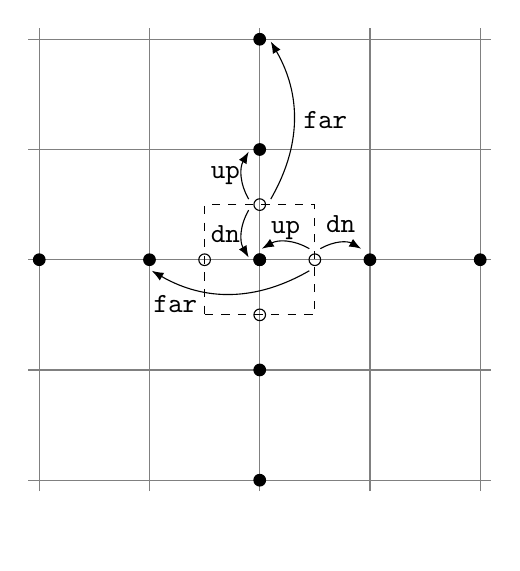
\begin{tikzpicture}[scale=1.4]
  \foreach \x in {-2.0,-1.0,0.0,1.0,2.0} {
      \draw[gray,thin] (\x,-2.1) -- (\x,2.1);
  }
  \foreach \y in {-2.0,-1.0,0.0,1.0,2.0} {
      \draw[gray,thin] (-2.1,\y) -- (2.1,\y);
      \filldraw (0.0,\y) circle (1.5pt);
  }
  \foreach \x in {-2.0,-1.0,0.0,1.0,2.0} {
      \filldraw (\x,0.0) circle (1.5pt);
  }
  \draw[dashed] (-0.5,-0.5) -- (0.5,-0.5) -- (0.5,0.5) -- (-0.5,0.5) -- cycle;
  \draw (0.5,0.0) circle (1.5pt);
  \draw (0.0,0.5) circle (1.5pt);
  \draw (-0.5,0.0) circle (1.5pt);
  \draw (0.0,-0.5) circle (1.5pt);
  %\node at (0.25,-0.25) {$V_{ij}$};
  % velocity direction entering cell
  %%\draw[-{Latex[length=2mm]}] (-1.6,0.7) -- (-0.1,0.05) node [midway,below] {$\mathbf{a}$};
  % E upwind decision:
  %\node at (0.7,-0.2) {$E$};
  \path[-{Latex[length=1.5mm]}] (0.45,0.1) edge [bend right] node [midway,above,yshift=-1mm] {\texttt{up}} (0.02,0.1);
  \path[-{Latex[length=1.5mm]}] (0.55,0.1) edge [bend left] node [midway,above] {\texttt{dn}} (0.92,0.1);
  \path[-{Latex[length=1.5mm]}] (0.45,-0.1) edge [bend left] node [midway,below,xshift=-7mm,yshift=1mm] {\texttt{far}} (-0.98,-0.1);
  % N upwind decision:
  %\node at (0.2,0.7) {$N$};
  \path[-{Latex[length=1.5mm]}] (-0.1,0.55) edge [bend left] node [midway,left,xshift=1mm] {\texttt{up}} (-0.1,0.98);
  \path[-{Latex[length=1.5mm]}] (-0.1,0.45) edge [bend right] node [midway,left,xshift=1mm] {\texttt{dn}} (-0.1,0.02);
  \path[-{Latex[length=1.5mm]}] (0.1,0.55) edge [bend right] node [midway,right] {\texttt{far}} (0.1,1.98);

  % generate padding at bottom
  \node at (0.0,-2.4) {\phantom{foo}};
\end{tikzpicture}
\end{document}
